\chapter{Interaktion}
Um aus der Visualisierung ausgewählter Strukturen und Informationen eine interaktive Projektion zu erzeugen ist es erforderlich Benutzereingaben zu erfassen und auszuwerten. Die Interaktion ermöglicht die Modifikation der Projektion und auch der damit gekoppelten Modelldaten.

\section{Detektion der Benutzerinteraktion}
Für die Erkennung der Benutzereingaben wird ebenfalls der Microsoft Kinect\red[TM] Sensor verwendet. Die Tiefeninformationen werden dabei in Form der erzeugten Punktwolken ausgewertet. Während der Benutzer das \kps{} in der einen Hand hält, kann die andere Hand verwendet werden um mit der Projektion zu interagieren. Auch andere Benutzer können mit dem System interagieren \red[sofern sie bei der Benutzereingabe die Rahmenbedingungen der Funktionsweise beachten].\\

Der implementierte Interaktionsansatz basiert auf der Analogie zu einem Laserpointer. Ziel ist es, dem Benutzer durch Zeigebewegungen die Interaktion mit der projizierten Modellumgebung zu ermöglichen.\\
Innerhalb des Softwaremoduls \mInteraction \red[Module schon beschrieben oder erst am Ende?] erfolgt dafür zunächst eine Distanz-Filterung der Punktwolke, da weit entfernte Messpunkte nicht aus der Benutzereingabe stammen, sondern die Umgebung abbilden. Alle Punkte außerhalb dieses Bereiches können für die weiteren Betrachtungen somit verworfen werden. Es ergibt sich damit der für die Benutzereingabe zur Verfügung stehende Interaktionsbereich, welcher in \abb{fig.intfov} dargestellt ist.\\
\red[xmin durch Hardware gegeben, Bereich dann parametrierbar, alles darüber (rot) wird verworfen\\]

\begin{figure}[!ht]
	\begin{center}
		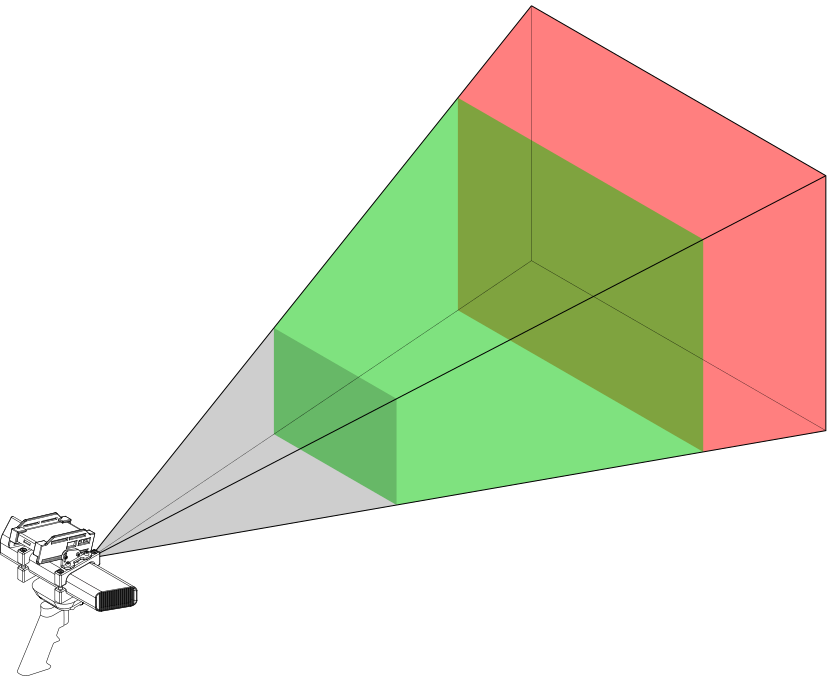
\includegraphics[scale=0.4]{interaktionsbereich}
		\caption{Möglicher Interaktionsbereich}
		\label{fig.intfov}
	\end{center}
	%\vspace*{-8mm}
\end{figure}

\red[Bemaßung?\\]

Basierend auf den verbleibenden Punkte wird anschließend eine Ebenendetektion nach \cite{Fischler1981} durchgeführt. Alle Punkte innerhalb eines definierten Abstandes werden daraufhin auf die \red[approximierte] Ebene projiziert, wodurch Messwertrauschen geglättet wird. Außerhalb der Ebene liegende Punkte werden für die weiteren Schritte aus der Betrachtung entfernt. Dazu gehören deutliche Ausreißer im detektierten Interaktionsobjekt sowie weitere Artefakte in der Punktwolke.\\

Um eine gleichmäßige Objektstruktur zu erhalten wird eine Hüllkurve um die verbleibenden Punkte gelegt und die vorhandene Struktur mittels einer äquidistanten Verteilung von Punkten angenähert. Aus dieser Hüllkurve wird der geometrische Schwerpunkt (Basis) sowie der vom \kps{} am weitesten entfernte Punkt (Spitze) bestimmt. Der Verbindungsvektor zwischen Basis und Spitze bildet damit die Zeigerichtung des Anwenders ab.\\
\red[\abb{fig.intdir}]

\begin{figure}[!ht]
	\begin{center}
		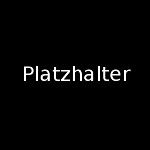
\includegraphics[scale=1.0]{spacer}
		\caption{Filterung der Punktwolke zur Bestimmung der Zeigerichtung - Subfigures: Punktewolke gesamt mit erkannter Ebene ; Projektion der Punkte auf Ebene und Entfernung von Artefakten ; Hüllkurve mit Centroid und Tip ; Erkannte Linie}
		\label{fig.intdir}
	\end{center}
	%\vspace*{-8mm}
\end{figure}

Um kleine unwillkürliche Bewegungen des Anwenders zu filtern wird der gleitende Mittelwert der Punkte bestimmt. Auch die Differenz zwischen zwei Punkten aus aufeinander folgenden Messungen wird überwacht, um zu große Sprünge in der Bewegung aufgrund von Fehldetektionen erkennen zu können.\\
Aufgrund des Implementierten Ansatzes wurde für die Kommunikation eine Nachrichtenstruktur definiert, welche die erkannte Linie abbildet. Das \mInteraction stellt die ermittelte Linie über diese Nachricht zur Verfügung und das \red[\mVisualization ?] empfängt diese.\red[ Module schon genannt?]\\

%Da die Kamera des Kinect Sensors auch von dem \mFovis verwendet wird besteht die Gefahr der Beeinflussung zwischen der Benutzereingabe und der lokalen Lokalisation. Um diese zu vermeiden sendet das \mInteraction Modul einen Befehl zum Pausieren der visuellen Odometrie sobald Punkte innerhalb des Interaktionsbereiches erkannt werden. Die visuelle Odometrie wird somit für die Dauer der Benutzerinteraktion unterbrochen. Sobald keine Punkte mehr innerhalb des Interaktionsbereiches detektiert werden, sendet das \mInteraction ein Signal zur Wiederaufnahme der visuellen Odometrie an das \mFovis .
Da die Kamera des Kinect Sensors auch zur Bestimmung der visuellen Odometrie verwendet wird besteht die Gefahr, dass die lokale Lokalisation durch die Benutzereingabe beeinträchtigt wird. Um dies zu vermeiden wurde eine direkte Kommunikation zwischen den beteiligten Modulen implementiert. Die visuelle Odometrie wird dabei unterbrochen, sobald Punkte innerhalb des Interaktionsbereiches erkannt werden. Endet die Interaktion, kann die visuelle Odometrie wieder aufgenommen werden.
Im Falle kleiner Posenänderungen während der Benutzereingabe ist die Lokalisation in der Lage die Veränderungen zu erkennen und die Pose im Anschluss an die Benutzerinteraktion zu aktualisieren.

\section{Erkennung von Befehlen}
Die Auswertung der auf Basis der Zeigebewegung ermittelten Linie erfolgt innerhalb des \red[\mVisualization]. Die Detektion der Linie erfolgte im Koordinatensystem der Kamera $\ks{K}$, so dass diese für die Auswertung zunächst über $\tmat{M}{K}$ in das Koordinatensystem der Karte $\ks{M}$ transformiert wird.\\

Um zu determinieren auf welches Modellobjekt der Benutzer gezeigt hat werden entlang der Linie alle Schnittpunkte mit den Modellen bestimmt. Dazu wird die Visualisierungsumgebung VTK verwendet, welche die Ermittlung von Schnittpunkten zwischen den Modellobjekten und Linien als Funktion zur Verfügung stellt. Aus den Schnittpunkten kann somit ermittelt werden, auf welches Objekt der Benutzer gezeigt hat. Die Auswahl eines Objektes, analog einer \glqq Klick\grqq -Aktion, erfolgt durch Überprüfung der Verweildauer des simulierten Zeigers auf dem Objekt.\red[ODER DURCH BUTTON!] Überschreitet diese einen definierten Grenzwert wird dies als Auswahlbefehl gewertet und das Objekt in den Zustand \textit{aktiv} versetzt. Durch Veränderung der Textur erhält der Anwender das visuelle Feedback, dass ein Objekt ausgewählt und in den neuen Status versetzt wurde (\abb{fig.intintersect}).\\

\begin{figure}[!ht]
	\begin{center}
		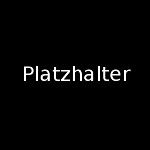
\includegraphics[scale=1.0]{spacer}
		\caption{Subfigures: Line intersection mit Modell und Abbildung des Laserpunktes - Aktivierung des Objektes}
		\label{fig.intintersect}
	\end{center}
	%\vspace*{-8mm}
\end{figure} 

Innerhalb der Modellumgebung können nun temporäre Interaktionsobjekte (\abb{fig.intarrows} \red[(a)]) eingeblendet werden, welche anschließend vom Benutzer ebenfalls über das zuvor beschriebene Funktionsprinzip ausgewählt werden können. Alle weiteren Modellobjekte werden während dieser Phase in den Status \textit{inaktiv} versetzt. Es ist somit immer nur ein Objekt der Modellumgebung \textit{aktiv}, wodurch für den Anwender eine klare Zuordnung der Interaktionsobjekte möglich ist.

\begin{figure}[!ht]
	\begin{center}
		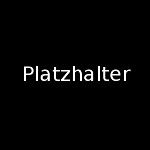
\includegraphics[scale=1.0]{spacer}
		\caption{Subfigures: Einblendung der Interaktionsobjekte und Auswahl durch Benutzer - Verschobenes Modell}
		\label{fig.intarrows}
	\end{center}
	%\vspace*{-8mm}
\end{figure} 

Durch Auswahl der Interaktionsobjekte ist der Benutzer in der Lage das aktuell als \textit{aktiv} gewählte Objekt innerhalb der Modellumgebung zu modifizieren. \abb{fig.intarrows} \red[(b)] zeigt dies am Beispiel der Translation des Modellobjektes. \red[Prinzipiell alle sechs räumlichen Freiheitsgrade möglich.]\\

Durch die Erkennung der Benutzereingabe können somit Objekte der Modellumgebung ausgewählt und bezüglich ihrer Pose modifiziert werden. Die Integration der Interaktion in die Visualisierung ermöglicht die direkte Modifikation der zugrunde liegenden Modelldaten. Das aktualisierte Modell kann abschließend gesichert werden wodurch eine Rückführung in den virtuellen Modellierungs- und Planungsprozess erreicht wird.


\red[Intersection sollte auch mit Modellumgebung möglich sein, damit der Pointer realistisch abgebildet wird!? Vielleicht Modell (obj) der Karte mit schwarzer Textur?]